\subsection{Overview}
The liaison system was verified utilizing automated testbenches. The testbenches uses VHDL assertions to notify the author if any
of the tests failed. In order to create a good and short but extensive testbench, we have built a collection of procedures that takes input, expected output
and expected system status after all input has been sent.

The test cases was divided into three blocks.
\begin{itemize}
\item The first test block consists of 8 tests that asserts the normal behaviour. It is done with some easy cases and a 2 cycle delay between inputs.

\item The second test block consists of 24 cases that at some point broke our logic.  tests where our design was likely to have flaws. During development, these tests were
triggered often, proving their value.

\item The third and last test block tests all possible microcontroller
  failure sequences. For each such sequence, it asserts that the
  correct data is voted and the correct status produced, and that the
  system functions correctly afterwards with all the microprocessors
  sending the same word for all 256 different words. The
  microcontrollers all sending the same word is also tested with no
  erroneous microcontrollers for each possible word. This block
  consists of 269 376 different test cases, and cover almost any
  possible state. The states that are not covered are those where one
  of the MCUs fails in the middle of the transaction, which are
  covered in the second block.
\end{itemize}

Since all permutations of failure sequences and all permutations of
valid input within these states were applied to the circuit during
simulation, we are confident that the Liaison System is working
correctly. We have also tested the circuit with a post-place and route
simulation verifying that the output is also correct with timing taken
into account\footnote{The timing simulation was done with iSim from
  Xilinx, synthesised with XST. Both tools are part of the ISE Design
  Suite}.

\subsection{Conformance with requirements specification}
This section explain the conformance with each point in the system requirements specification.
\begin{enumerate}
    \item{\textbf{The Liaison Interface}} \hfill\\
        Our implementation of the Liaison System follows the signaling interface given by the requirements\cite{task}.

    \item{\textbf{Voting}} \hfill\\
        The Voting algorithm has been tested and confirmed to be working. This was done by enumerating all
        permutations of input and state, and then check the Voters result against expected output using
        VHDL assertions.

    \item{\textbf{Error tagging}} \hfill\\
        The error tagging is not specified in the requirements, but is nessesary in our implementation to
        achieve correct System Status bits and correct Voting. The error tagging was tested with the same
        tests as the Voting algorithm and does conform with the expected behaviour.

    \item{\textbf{System status}} \hfill\\
        The System Status is needed to tell the receiver about the health of the microcontrollers. Since
        there exists a direct mapping between the Error tagging and the System Status, this is also
        included in the same tests as Error tagging and Voting.

    \item{\textbf{Error correcting code}} \hfill\\
        The Error correcting code is a specific part of the requirements\cite{task}. The module was tested by writing
        a testbench function that generates (15,11) Hamming Code with SECDED from an 11-bit word. This
        procedure was added to the enumerated tests from the Voter-test such that for each input, the testbench
        would automatically expect a specific ECC. If the ECC from the function was not equal to the output
        of the Liaison, assertions were raised to the tester. Since the soft function agrees with the simulated
        hardware, we are certain that the ECC-module works as specified in the requirements. The ECC-generating
        software function can be found in \autoref{apx:ecc}.

    \item{\textbf{Reset behaviour}} \hfill\\
        On reset, The Liaison is set back to inital state on next clock cycle. The reset is stricly synchronous,
        as stated in the requirements\cite{task}, and is thus only read on rising edge of the clock. We have
        tested that reset works for any final state when a data sequence finished, but we have not tested the
        behavoiur of a reset in the middle of a transmission. By simple code inspection, we see that the
        reset is not aware of current system status, but simply sets all the state variables back to initial
        state. That means that after a reset signal is asserted along with rising edge of the clock, the system
        will not process data until a new {\ttfamily di\_ready}.

    \item{\textbf{System consitency}} \hfill\\
        Since all possible inputs for both the Voter and the ECC module has been exhaustively tested, and 
        since very little of the internal system logic is dependent on both system status and current bit-position,
        we are sure that the exhaustive tests run on the Voter and the ECC module is sufficient to conclude that 
        the entire system is consitent with the requirements. All enumerations of fail states have been tested, all combinations
        of input to the ECC module have been tested, and the Output Multiplexer cares only about current output bit position,
        and is thus also exhaustivly tested.

    \item{\textbf{New data after $11+m$ cycles}} \hfill\\
        Most of the test cases send data directly after previous data word was correctly received, and we have
        added a few tests where there is a delay between each received word. Thus, the system works as required,
        and is able to receive new data after $11+m$ clock cycles. This is shown in \autoref{fig:timing}

\end{enumerate}

\begin{figure}
    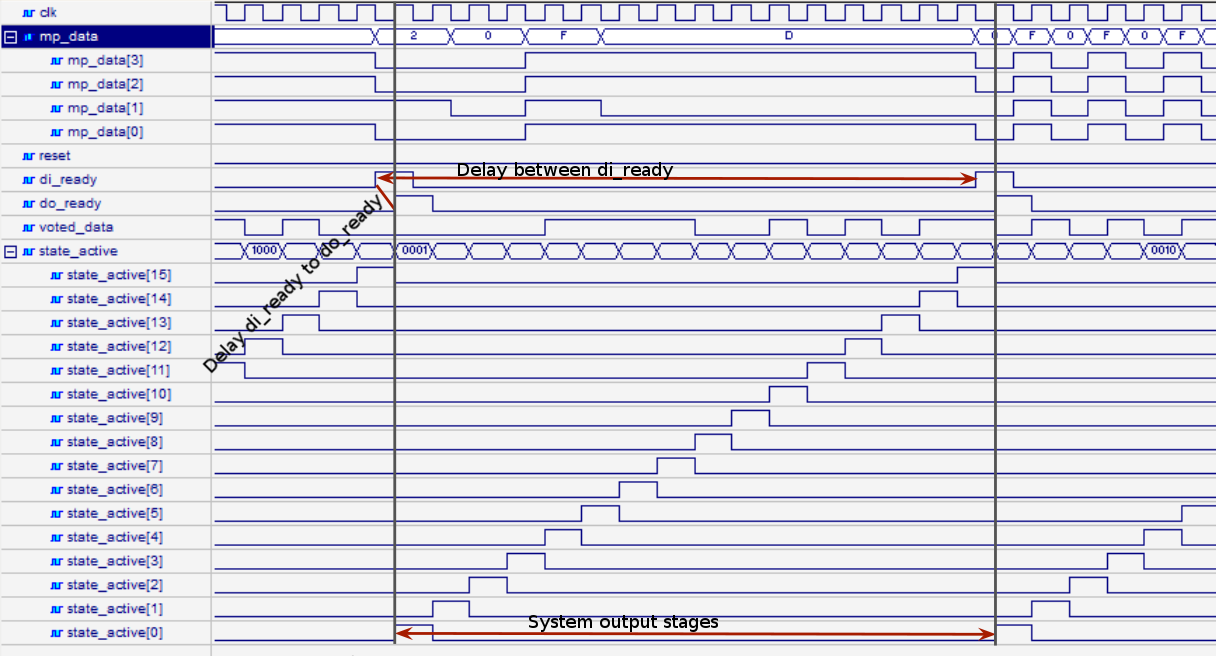
\includegraphics[width=\textwidth]{tests/timing}
    \caption{Timing diagram of data received with minimum delay}
    \label{fig:timing}
\end{figure}
